
\chapter{Related Work}
\label{related}


This thesis focuses on extending the DDSP-based autoencoder by \cite{ddsp} aiming to create a single model that can quickly learn to mimic diverse sounds from little data.
The first part of this section contains a detailed description of this baseline model.
In the second part, other machine learning models that can learn to synthesize natural data are presented.



\section{Differential Digital Signal Processing (DDSP)}
An audio signal is not an arbitrary time series of air pressure values: we know that sound is often produced by vibrating objects, or gets perceptually relevant features from filters being applied to a base signal.
If a note is played on an instrument such as a violin, the strings vibrate with a fundamental frequency $f_0$ and integer multiples of that frequency: their harmonics.
A recording of sound in its raw form is called the waveform, and spectral information can be made available using a Short-Time Fourier Transform (STFT).
Our perception relies mostly on spectral features of sound and much less on absolute air pressure values or the phase of a sound. For this reason, spectrograms are such a popular preprocessing step for tasks that involve audio feature extraction. \newline
However, since a real-valued spectrogram contains no information about the phase of the sound, it is not perfectly suited for audio generation.
For waveform generation, many different types of synthesizers exist that can create a wide variety of sounds. \newline
Motivated by these observations, \citet{ddsp} proposed DDSP as a way of incorporating this knowledge about audio into neural network architectures.
Specifically, they built an autoencoder for monophonic recordings of musical instruments.
Its encoder extracts the fundamental frequency, the loudness, and optionally an additional latent variable $z$ from the waveform. The decoder reconstructs the signal by controlling a harmonic plus filtered noise synthesizer.
The architecture is shown in \Cref{ddsp-schema}.\newline


\begin{figure}
    \caption{Baseline DDSP architecture}
    \label{ddsp-schema}
    \begin{center}
        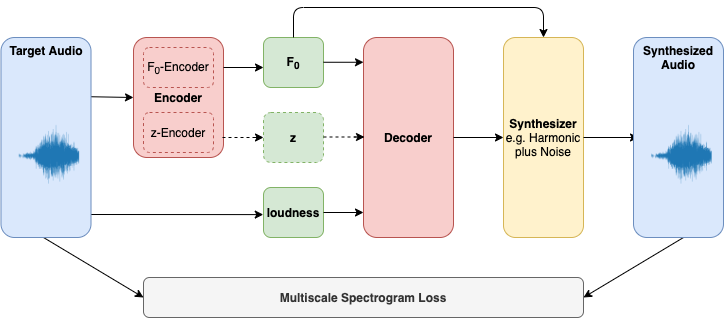
\includegraphics[width=400px]{schema/ddsp.png}
    \end{center}
        {\small The encoder computes $f_0$ using a pretrained model called CREPE and an additional latent variable $z$. From that, the decoder reconstructs the original audio by controlling a harmonic plus filtered noise synthesizer.
        }
\end{figure}

A harmonic plus noise synthesizer consists of two separate modules: a harmonic synthesizer and a filtered noise synthesizer.
Harmonic audio occurs when an object can vibrate freely: a guitar string oscillates with a fundamental frequency and multiples of that.
However natural signals often contain at least a certain amount of noise and other non harmonic elements, which is why a filtered noise synthesizer is added. \newline
The harmonic synthesizer mixes sine waves with instantenous frequency $f_k = k * f_0$ according to a harmonic distribution $h \in \mathbb{R}^H$, where $H$ is the number of harmonics and $h$ is an output of the decoder. The signal is then scaled by the total amplitude $a$, such that the waveform at time $t$ is computed as:
\begin{equation}
    \begin{split}
    s_{harmonic}(t; f_0, h, a) = a_t \sum_i h_i \sin(2 \pi i F_{0, t})
\end{split}
\end{equation}
where $F_{0, t}$ is the unrolled phase
\begin{equation}
    \begin{split}
    F_{0, t} = \frac{1}{sr} \sum_{i = 0}^{t} f_{0,i}
\end{split}
\end{equation}
An illustration of this synthesizer is shown in \Cref{fig:harmonic}. \newline

\begin{figure}
    \centering
    \begin{minipage}[b]{0.45\textwidth}
        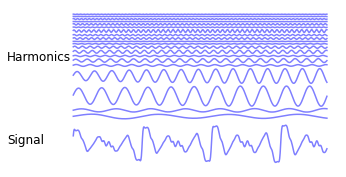
\includegraphics[width=\textwidth]{figures/harmonic_wave.png}
        \small A harmonic synthesizer synthesizes a signal that is made up of scaled sine waves with frequencies that are integer multiples of $f_0$. This waveform corresponds to 31 milliseconds of audio.
      \end{minipage}
      \hfill
      \begin{minipage}[b]{0.45\textwidth}
        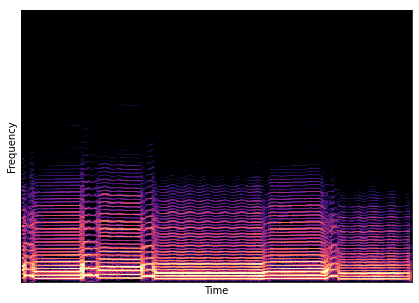
\includegraphics[width=\textwidth]{figures/harmonic_spectro.png}
        \small The spectrogram of 4 seconds of a harmonic waveform.
    \end{minipage}
    \caption{Harmonic Synthesizer} 
    \label{fig:harmonic}   
\end{figure}

The filtered noise synthesizer is a band-pass filter applied to white noise - here, the neural network predicts time distributed noise magnitudes for a number of frequency bands. A waveform and a spectrogram of filtered noise are shown in \Cref{fig:filtered_noise}. \newline

\begin{figure}
\centering
\begin{minipage}[b]{0.45\textwidth}
    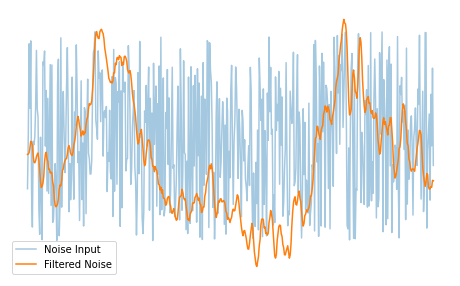
\includegraphics[width=\textwidth]{figures/filtered_noise_wave.png}
    \small A filtered noise synthesizer receives random white noise as an input and applies frequency-band pass filters to it to generate a waveform. This waveform again corresponds to 31 milliseconds of audio.
  \end{minipage}
  \hfill
  \begin{minipage}[b]{0.45\textwidth}
    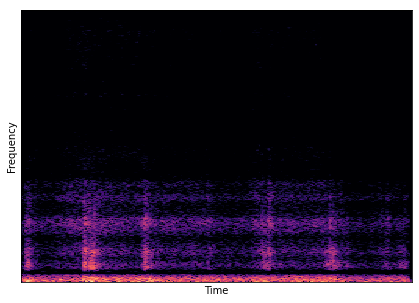
\includegraphics[width=\textwidth]{figures/filtered_noise_spectro.png}
    \small The spectrogram of 4 seconds of audio output of a filtered noise synthesizer.
\end{minipage}
\caption{Filtered Noise Synthesizer}
\label{fig:filtered_noise}
\end{figure}



The organization of the latent space into these perceptually relevant variables and the use of synthesizers induce a structural bias on the model that is well suited for modeling monophonic audio.
Furthermore, the prior that our perception depends mostly on spectral features is reflected by the use of a multi-scale spectrogram loss function \citep{wang_neural_2019}.


Using $f_0$, loudness and $z$ as the structure for the latent space was first proposed by \citet{hantrakul_fast_2019-1} together with a WaveRNN architecture, motivated by the success of TTS systems with informative local conditioning such as mel spectrograms.
Hierarchical Timbre Painting (HPT) \citep{michelashvili_hierarchical_2020} use the same latent representation together with a ParallelWaveGAN \citep{yamamoto_parallel_2020} architecture in the decoder.
While their sound samples are impressive and arguably a slight improvement over the DDSP baseline, I found exchanging the DDSP decoder by a Parallel WaveNet architecture to hurt performance in my initial experiments, if additional tweaks that require huge implementation efforts were not used: HPT is trained to upsample a low-resolution signal multiple times, requiring additional discriminators for each upsampling step. Training a baseline DDSP architecture is much more convenient as it trains only a single model, without the need for advanced training schedules to train different upsampling models and their respective discriminators.



Follow up work on DDSP by \citet{hayes_neural_nodate} add learned neural waveshaping units (NEWTs) to the synthesizer. These units get harmonic oscillators corresponding to $f_0$ as input, which are fed to a multi-layer perceptron (MLP) that uses sine waves as nonlinear activations.
The MLP additionally gets time distributed audio features $z$ as input and resembles a SIREN with a hypernetwork \citep{siren}.
Using this approach allows very fast and high-quality audio re-synthesis. However, just like the original DDSP autoencoder, one model has to be trained for each target timbre. The suggested improvements of this work can potentially be combined with the methods evaluated in this thesis. \newline

Related work by \citet{liu_neural_2020} similarly use DSP-inspired techniques for neural vocoding: their model is conditioned on $f_0$ and additional log mel-spectrogram features $z$, and learns to control linear time-varying filters (LTVs) in order to generate speech.
The network predicts LTVs which are then applied to a periodic impulse train with frequency $f_0$, and to stochastic noise. LTVs applied to an impulse train yield harmonic signals which appear in voiced speech, and LTVs applied to noise add non-harmonic parts - just like the filtered noise synthesizer used in the baseline DDSP architecture.
Besides applying it to a different problem, namely speech synthesis, the main difference is therefore the decoder architecture.
The techniques explored in this thesis all use the same decoder as the baseline DDSP model. However, they don't necessarily depend on it and can therefore be combined with alternative decoder/synthesizer architectures. \newline
Another work that uses DDSP for vocoding is \citet{mccarthy_hooligan_2020}: here, a WaveNet is used on top of the individual harmonics and noise outputs of a DDSP autoencoder.


\section{Other Approaches to Audio Modelling}
% Wavenet
\textbf{WaveNet} A major breakthrough for audio generation were autoregressive models like WaveNet \citep{WaveNet} and WaveRNN \citep{kalchbrenner_efficient_2018}, which are able to learn conditional and unconditional audio synthesis and the task of transforming text to speech (TTS).
However, due to their autoregressive sampling, training and inference are extremely slow and due to the lack of any audio-specific bias, everything that is typical for sound has to be learned from scratch.
These models are trained to maximize the log-likelihood of the audio data by factorizing
\begin{equation}
    p(x) = p(x_1) \cdot p(x_2|x_1) \cdot \dots \cdot p(x_n|x_1, \dots , x_{n-1})
\end{equation}
where $x = (x_1, \dots, x_n)$ is the audio data as a waveform.
In order to sample from the model, one forward pass is necessary to obtain $x_1$, which is send fed back into the network to obtain $x_2$ and so on. Audio is typically sampled with at least 16000 Hz, which corresponds to the number of forward passes necessary to generate a single second of audio.

Non-autoregressive variants of it such as Parallel WaveNet \citep{oord_parallel_2017} improve the inference speed, but still require huge amounts of training data and GPU time.

Other models like VQ-VAE and VQ-VAE-2 \citep{vqvae} \citep{vqvae2} use a WaveNet as a building block, and additional modules to learn long-range dependencies.





% Diffusion
\textbf{Diffusion based models} Diffusion based models recently became very popular for image generation \citep{dhariwal_diffusion_2021}.
For audio generation, they also show promising results: \citet{kong_diffwave_2021} introduced DiffWave, a vocoder that generates audio of spoken words from a mel-spectrogram.
Diffusion models are trained to revert a process called diffusion, where noise is repeatedly added to a signal $x_{(0)}$.
After a fixed number of steps $T$, the signal $x_{(T)}$ is approximately gaussian distributed, which means that using $T$ denoising steps, a random vector $\hat{x}_{(T)} \sim \mathcal{N}(\mu,\,\sigma^{2})$ can be transformed into a an audio signal $\hat{x}_{(0)}$.
More precisely, the model approximates the distribution of the signal at the previous time step, given $x_{(t)}$ as:
\begin{equation}
    \begin{split}
p(x_{(t-1)} | x_{(t)}, t, C) \sim \mathcal{N}(\mu_{(t)},\,\sigma_{(t)}^{2}) \\
\mu_{(t)},\,\sigma_{(t)} = f(x_{(t)}, t, C)
\end{split}
\end{equation}
where $C$ is a control signal, e.g. features of a mel-spectrogram, and $f$ is the forward pass of the neural network. \newline


\textbf{GAN-based Approaches}
WaveNet variants and diffusion-based models optimize the likelihood of the waveform. As an alternative to this, also GAN-based approaches can be used to model audio. 
Parallel WaveGAN \citep{yamamoto_parallel_2020} and HPT \citep{michelashvili_hierarchical_2020} use generators that work in the waveform domain together with dilated convolutional layers, similar to the ones used in WaveNet. GANsynth \citep{engel_gansynth_2019} uses an invertible spectral representation of the audio. \newline
In early experiments, I tried training a DDSP-autoencoder with a GAN objective but found training difficult. The discriminator struggles to differentiate between the real and generated audio even if it is trained for many more steps than the generator.

% Music generation
\textbf{Jukebox} The current state-of-the-art in music generation is Jukebox \citep{jukebox}. It uses stacked transformers to learn the structure of music on multiple time-scales, and a VQ-VAE to generate music from latents.
For such an approach, it is nice to have a low-level model with an encoder: in that case, the latent representation of natural music can easily be computed and used as the ground truth for another model that learns the next layer of abstraction. \newline
The line of work on DDSP based architectures provides a potential alternative to the VQ-VAE within Jukebox.
A limitation is, however, that the currently available DDSP-based architectures only work for monophonic audio.
An encoder that controls multiple synthesizers to model polyphonic audio would be necessary to lift DDSP towards a general-purpose audio autoencoder.
Creating a model that can capture all different kinds of monophonic audio is a first necessary step towards building a general-purpose polyphonic model, and this challenge is addressed in this thesis. \newline




% - WaveNet, ParallelWaveGAN, hierarchical timbre painting
% - vqvae
% - diffusion models: \citep{kong_diffwave_2021}
% - flow based: \citep{prenger_waveglow_2019}
% - gan based: DCGAN both on spectros and waveforms: \citep{donahue_adversarial_2019}
% - gansynth \citep{engel_gansynth_2019}: on invertible spectral representation (including the phase)









% - Closely related to DDSP, timbre painting:
%     (f0, loudness, timbre, room acoustics) -> waveform
%     - schema unified framework
%     - DDSP: controlling synthesizers
%     - Timbre Painting: minimalistic synthesizer + upsamplers with adversarial loss; ParallelWaveGAN
%     - Scope: monophonic audio
% - Related by application:
%     - f0 detection: CREPE, others?
%     - audio source separation: ?
% - General-purpose waveform generative architectures:
%     - WaveNet
%     - VQ-VAE to extend length in which WaveNet can generate
%     - DiffSynth (read their related work part again)
%     - flow-based?
% - Spectrogram based architectures:
%     - ?
% - Generative music
%     - often in symbolic domain: midi: music-transformer, midinet, vaeseq + midi
%         - midi is not general-purpose
%         - less training data available
%     - jukebox



% \begin{figure}
%     \label{timbrepainting-schema}
%     \begin{center}
%         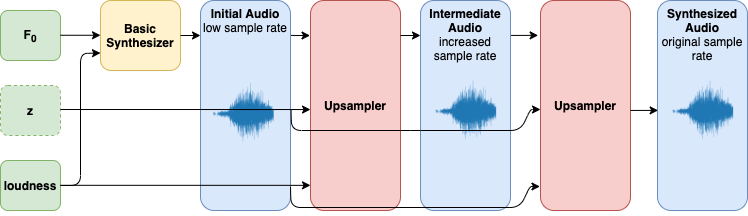
\includegraphics[width=400px]{schema/timbre_painting_audiodecoder.png}
%         \caption[Timbre Painting Decoder]%
%         {\small The decoder of \cite{timbrepainting} is a ParallelWaveGAN.}
%     \end{center}
% \end{figure}

% \begin{figure}
%     \label{unified-schema}
%     \begin{center}
%         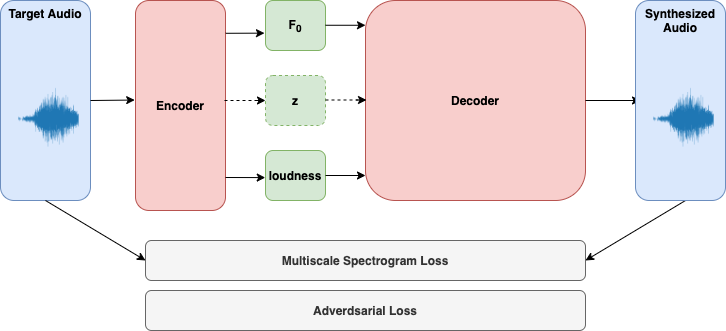
\includegraphics[width=400px]{schema/ddsp_and_timbrepainting.png}
%         \caption[A unified schema for monophonic audio autoencoders]%
%         {\small DDSP and timbre painting represent audio as f0, loudness and optionally a timbre vector.}
%     \end{center}
% \end{figure}